\documentclass{article}
\usepackage{amsmath, amssymb, mdwlist, graphicx, hyperref}
\usepackage{listings,color}
\usepackage{wrapfig}
\usepackage[usenames,dvipsnames]{xcolor}
\definecolor{gray}{rgb}{0.97,0.97,0.97}
\lstset{%
language=C,%
%backgroundcolor=\color{gray},
emph={putpixel},
emphstyle=\bf,
tabsize=4,
framesep=5pt,
mathescape=true,
xleftmargin=0.1cm,
xrightmargin=0.1cm,
frame=lines,
%basicstyle=\ttfamily,
%keywordstyle=\color{Blue},
%commentstyle=\color{OliveGreen},
%stringstyle=\color{MidnightBlue},
columns=flexible,
%showstringspaces=false
}

\newcommand{\mpar}[1]{\marginpar{\textit{#1}}}
\newcommand{\norm}[1]{\Vert #1 \Vert}
\DeclareMathOperator{\argmax}{argmax}
\DeclareMathOperator{\argmin}{argmin}
\newenvironment{solution}{\paragraph{Solution.}$\,$ }{\vskip 3mm\hrule}
\newenvironment{exercise}[2]{\paragraph{Exercise #1 (#2pt).} }{
\medskip}
\newcommand{\bbR}{\mathbb{R}}
\newcommand{\bw}{\mathbf{w}}
\newcommand{\bx}{\mathbf{x}}
\newcommand{\bd}{\mathbf{d}}
\newcommand{\bb}{\mathbf{b}}
\newcommand{\by}{\mathbf{y}}
\newcommand{\bzero}{\mathbf{0}}
\newcommand{\bz}{\mathbf{z}}
\newcommand{\bSigma}{\mathbf{\Sigma}}
\newcommand{\bp}{\mathbf{p}}
\newcommand{\bP}{\mathbf{P}}
\newcommand{\bm}{\mathbf{m}}
\newcommand{\bc}{\mathbf{c}}
\newcommand{\bM}{\mathbf{M}}
\newcommand{\bV}{\mathbf{V}}
\newcommand{\bK}{\mathbf{K}}
\newcommand{\bD}{\mathbf{D}}
\newcommand{\bA}{\mathbf{A}}
\newcommand{\bX}{\mathbf{X}}
\newcommand{\bY}{\mathbf{Y}}
\newcommand{\bR}{\mathbf{R}}
\newcommand{\bI}{\mathbf{I}}
\newcommand{\bS}{\mathbf{S}}
\newcommand{\bT}{\mathbf{T}}
\newcommand{\balpha}{\boldsymbol{\alpha}}
\newcommand{\pt}[2]{\left(\begin{array}{c}#1\\#2\end{array}\right)}

\begin{document}
\title{MTAT.03.015 Computer Graphics (Fall 2013)\\
Exercise session IX: Shadows}
\author{Konstantin Tretyakov, Ilya Kuzovkin}
\date{November 4, 2013}
\maketitle

The standard graphics pipeline is a very efficient algorithm for rendering complex scenes -- this is the reason why it is the primary (if not the only) method used nowadays in high-performance graphics, such as games or interactive visualization.

However, as the scene in this algorithm is rendered on a strictly ``local'' polygon-by-polygon basis, implementing any effects related to global light propagation, such as shadows, reflections, transparency and various kinds of light scattering from one object to another, is increasingly hard or cumbersome. In this exercise session we shall study the three most popular algorithms for implementing shadows in the standard graphics pipeline framework. While working on them, think how each of them solves the problem of introducing ``global'' light interaction into an otherwise purely local approach in its own way.

As usual, the code base is provided in \texttt{practice09.zip} archive on the course website or via the course github page. Download, unpack and open it. You will need to submit your solution as a zipped archive file.

\section{Projective Shadows}
Open the project \verb#1_ProjectiveShadows# and study the code. The main file of the project is \verb#projective_shadows.cpp#, which presents the (now hopefully very familiar to you) structure of a GLUT application. The \verb#display# function renders a simple scene with three ``walls'' (a floor and two walls, to be more precise), two ``objects'' (which are actually cubes) and two light sources. To simplify the code, some of the functionality has been separated into the file \verb#scene_primitives.cpp#.  You should not need to look much into that file, in principle, but you should at least study the \verb#scene_primitives.h# header to understand what it provides.

\begin{exercise}{1}{0.5} Complete the \verb#display# function by adding code that renders projection shadows for both cubes from both light sources onto the walls and the plane. An example is provided to get you started. Note that your main tool here is the \verb#shadowMatrix(light, plane, offset)# function (provided in \verb#scene_primitives.h/.cpp#). This function constructs a projection matrix with \verb#light# as the center of projection, and \verb#plane# as the projection plane. Multiplication by this matrix ``squishes'' all primitives onto the projection plane. The projection plane is specified as a four-component vector $(a, b, c, d)$. This vector provides the coefficients of the implicit plane equation
$$
ax + by + cz + d = 0,
$$
For example, for the floor plane ($z = 0$) the implicit equation is 
$$
0x + 0y + 1z + 0d = 0,
$$
i.e. the corresponding vector is \verb#{0, 0, 1, 0}#. You will need to provide plane equations for the right wall $(x = 4)$ and the back wall $(y = 4)$ as well.

Finally, the \verb#offset# parameter adds a tiny offset to the ``squished'' object shadow along the normal to the plane $(a, b, c)$. This prevents depth-buffer related artefacts (set offset to $0$ to observe them).
\end{exercise}

Note that despite their overall conceptual simplicity, projective shadows are quite limited in what you can achieve with them: objects do not cast shadows on each other, and the computation scales linearly with the number of planes that should receive shadows.

A popular version of the same idea is that of \emph{projective textures}\footnote{\url{http://en.wikipedia.org/wiki/Projective_texture_mapping}}, where some texture image is projected onto geometry from the light source center (like a projector would)\footnote{Note that the \texttt{GL\textunderscore EYE\textunderscore LINEAR} texture coordinate generation mode with default parameters, that you had a chance to briefly see in the last practice session, is essentially an orthogonal projection of the texture from the viewer onto the objects in front of him.}. If the texture contains pre-rendered shadow silhouettes this can be used as a simple shadow rendering algorithm (sometimes referred to as \emph{projective texture shadows}).


\section{Stencil Shadows}
A much better algorithm for real-time shadows is the \emph{stencil shadow} algorithm, most well known for its use in the game Doom III. The idea of the algorithm is quite well described in the corresponding Wikipedia article\footnote{\url{http://en.wikipedia.org/wiki/Shadow_volume}}.

\begin{exercise}{2}{1}
Open the project \verb#2_StencilShadows#. It has the same structure and uses the same geometry as the previous exercise. Modify the \verb#display# function to implement the stencil shadow algorithm. The main complication of the algorithm is the rendering of the shadow volumes, but this functionality is already provided for you in the \verb#Cube::draw_shadow_volume()# function. Follow the instructions provided in the comments in the code to complete the algorithm.
\end{exercise}

\begin{exercise}{3*}{0.5}
You should note that the shadows you obtained in the last exercise are actually incorrect: shadows from two different light sources are ``merged'' into an equally gray area, whereas in reality the region that is in shadow with respect to both light sources must be darker than the one where just one light source is seen. Indeed, a correct implementation of stencil shadows requires preparing a separate stencil buffer for each light source, rendering just the lighting component for that particular light source, and aggregating the resulting pixel values using blending or accumulation buffer. Implement this.

Hint: You might want to sacrifice sRGB-conversion for the sake of simplicity of implementation. In other words, a solution without proper gamma correction is acceptable for sake of grading in this exercise.
\end{exercise}

\section{Shadow Mapping}
Finally, probably the most popular way of implementing real-time shadows nowadays is \emph{shadow mapping}. The idea is to render the scene from the ``viewpoint of the light source'', saving the resulting depth buffer into a texture. That texture can then be used to check for any pixel whether it is occluded from the light source or not. Again, a fairly clear description of the technique is provided in Wikipedia\footnote{\url{http://en.wikipedia.org/wiki/Shadow_mapping}}.

\begin{exercise}{4}{2.5}
Open the project \verb#3_ShadowMaps# and study the\\ \verb#shadow_maps.cpp# file (in particular the \verb#display# function). The core shadow mapping algorithm logic is already implemented there. Your task is to complete the implementation by providing the appropriate fragment shader code in \verb#shadowmap.frag.glsl#. The comments in the fragment shader will hopefully provide enough guidance. 

Note that the shadow map texture only applies to fragments that fit into the view frustum of the corresponding light source. Everything outside that frustum has to be assumed to be either constantly lit, or be constantly in shadow, depending on your preference. In the former case shadows simply won't work outside of the view frustum. In the latter case the light sources will resemble a kind of ``square'' directional lights, and you would get a result like the following:

\begin{center}
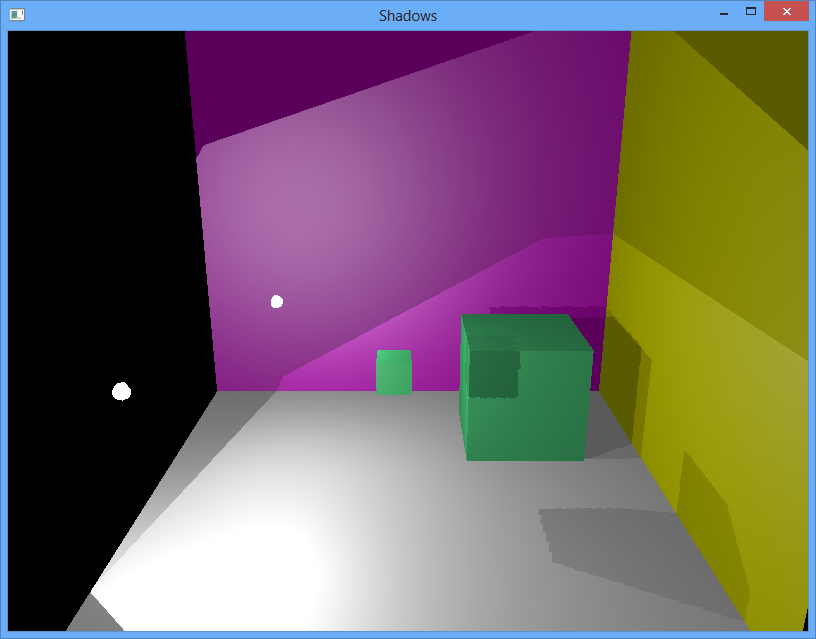
\includegraphics[width=0.7\textwidth]{shadow_maps.png}
\end{center}

Most probably your first working implementation will produce an artifact known as ``shadow acne''\footnote{\url{http://msdn.microsoft.com/en-us/library/windows/desktop/ee416324(v=vs.85).aspx}}:
\begin{center}
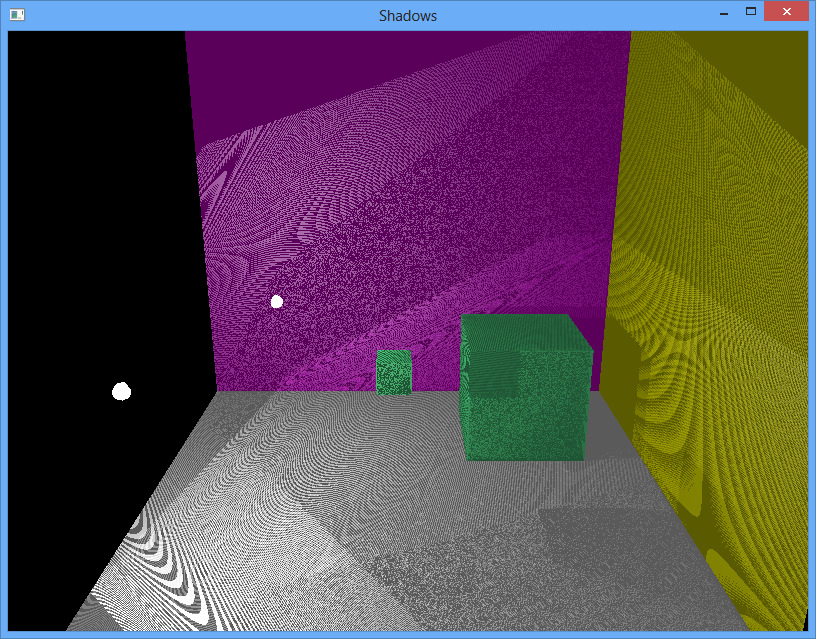
\includegraphics[width=0.7\textwidth]{shadow_acne.png}
\end{center}
It stems from having code like the following somewhere in your shader:
\begin{verbatim}
 if (current_depth_value <= texture_depth_value)
     c += blinn(gl_LightSource[i]); // The fragment is lit
\end{verbatim}
The artifact is due to limited number of samples in the depth texture and floating point discrepancies. Whenever the surfaces are lit, the values of \verb#current_# \verb#depth_value# and \verb#texture_depth_value# should, ideally, be strictly equal. However, due to the fact that \verb#texture_depth_value# is usually obtained via some kind of bilinear interpolation from the texture and \verb#current_depth_value# is computed through matrix multiplication, floating point discrepancies creep in and the equality is rarely exact: for some pixels one value is slightly greater, for other slightly less, which leads to the observed effects.

The fix is simple: add a small offset to the pixel's depth.
\begin{verbatim}
 if (current_depth_value - offset <= texture_depth_value)
     c += blinn(gl_LightSource[i]); // The fragment is lit
\end{verbatim}

When the offset is too large, however, gaps will start to appear between the objects and their shadows, and you don't want this to happen either.
\end{exercise}

\begin{exercise}{5*}{0.5}
For even nicer shadow mapping, it is possible to use GPU-s built-in capabilities for working with shadow maps. This will result in both cleaner code and better texture sampling, somewhat reducing aliasing artifacts. Try doing it:
\begin{enumerate}
\item Change the type of \texttt{shadowMapTexture}$k$ variables from \texttt{sampler2D} to \texttt{sampler2DShadow}.
\item Now, rather than accessing them as textures via the \texttt{texture2D} function, you will need to use the \texttt{shadow2D} function, which takes as input the shadow map texture and a three-dimensional point. It performs the whole shadow test (using $(x, y)$ to look up the depth value in the texture and $z$ to compare against), and returns nonzero value(s) if the shadow test passes, i.e. the corresponding point is not in shadow. You should not even need to worry about offsets and shadow acne\footnote{As long as you specify \texttt{GL\textunderscore LINEAR} filtering mode for your textures, at least}.
\item Moreover, there is also a \texttt{shadow2DProj} texture access function, which directly accepts four-dimensional homogeneous coordinates (so that you do not need to perform perspective division). You cannot immediately feed clip-space coordinates to it, however. As all other texture access functions, it expects coordinates scaled to texture-space range, i.e. $x, y, z$ must be in range $[0, 1]$ rather than $[-1, 1]$. The rescaling from clip-space homogeneous coordinates into the texture-space range can be done using the matrix
$$
\left(\begin{matrix}0.5 & 0 & 0 & 0.5\\
0 & 0.5 & 0 & 0.5 \\
0 & 0 & 0.5 & 0.5 \\
0 & 0& 0& 1\end{matrix}\right)
$$
\item Finally, performing the whole computation in the fragment shader is inefficient. Instead, we should compute the shadow map coordinates for each vertex in the vertex shader and simply use the interpolated values in the frament shaders\footnote{Notice that this means you will be doing a perspective-correct interpolation with respect to a perpective projection, that is \emph{different} from the one used to render the scene. Think how this is only possible due to homogeneous coordinates.}
\end{enumerate}
To get points for this problem implement the changes suggested above. Make use of the \texttt{shadow2DProj} function and perform all shadow coordinate computations (i.e. the corresponding matrix multiplications) in the vertex shader\footnote{At this point it becomes possible to make the code added to the fragment shader be a ``one-liner'' of the form \texttt{for(something) if (long condition) c += blinn(gl\textunderscore LightSource[i]);} The condition is the shadow map test.}.
\end{exercise}

Being able to understand and implement shadow maps is generally a good indicator that you have mastered the core concepts behind the standard graphics pipeline.

\end{document}
